\documentclass[a4paper,12pt]{article}
\usepackage{graphicx} % Required for inserting images
\usepackage{color}
\usepackage[UTF8]{ctex}
\usepackage{amsmath}
\usepackage{tabularray}



%\newcommand{\upsite}[1]{\textsuperscript}{cite{#1}}

%\bibliographystyle{unsrt}
\begin{document}
\begin{figure}[t]
    
\includegraphics[width=0.2\textwidth]{ouc.jpg}
\end{figure}

\title{实验报告}
\author{单衍喆 }
\date{2024-9-6}
\maketitle

\pagenumbering{roman}
\text{GitHub地址:https://github.com/Venusss1/course.git}
\tableofcontents
\newpage
%\pagenumbering{arabic}


\section{\underline{\color{blue}实验内容}}

\begin{enumerate}
    \item \textbf{Shell工具和脚本}
    \item \textbf{文档编辑工具Vim}
    \item \textbf{数据整理}
\end{enumerate}

\section{\underline{\color{blue}实验设计}}
\subsection{\color{red}Shell工具和脚本}

\subsubsection{\color{green}Linux系统环境配置}
\begin{enumerate}
    \item 下载安装VMware Workstation
          \begin{figure}[htbp]
              \centering
              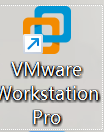
\includegraphics[width=0.2\textwidth]{VMware.png}
              \caption{VMware}
              \label{VMware}
          \end{figure}
    \item 下载Ubuntu系统文件
    \item 载入系统文件\\
配置网络和系统设置

\end{enumerate}
\subsubsection{\color{green}基本命令}

\begin{table}[h]
    \centering
    \caption{\color{green}基本命令}
    \begin{tblr}{
            cell{2}{1} = {c,fg=cyan},
            cell{3}{1} = {c,fg=cyan},
            cell{4}{1} = {c,fg=cyan},
            cell{5}{1} = {c,fg=cyan},
            vline{2} = {1-5}{},
            hline{1-2} = {-}{},
        }
        命令 & \textsf{作用}      \\
        echo & \textsf{标准输出}      \\
        man  & \textsf{查看帮助} \\
        chmod & \textsf{修改权限}      \\
    \end{tblr}
\end{table}
\newpage
\subsubsection{\color{green}环境变量}
env 可查看当前系统中所有环境变量\\
env PATH 可以查看特定PATH的值
\begin{figure}[h]
    \centering
    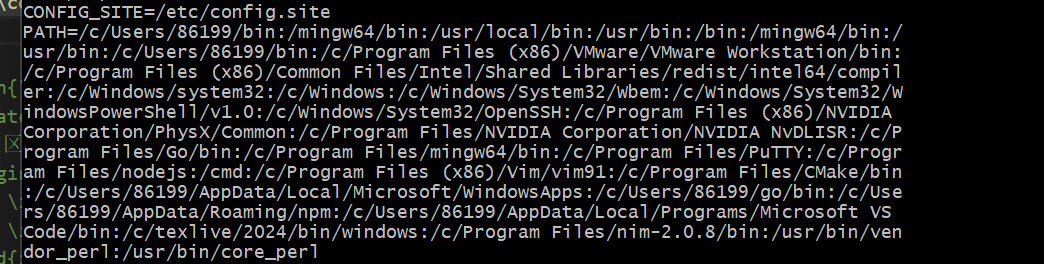
\includegraphics[width=1\textwidth]{path.png}
    \caption{PATH}
\end{figure}


\subsubsection{\color{green}文件操作}
\begin{itemize}
    \item pwd 展示当前目录下所有文件
    \item cd 切换目录
    \item ls 查看当前目录下所有文件
    \item mv 重命名和剪切文件
    \item cp 拷贝文件
    \item mkdir 新建文件夹
    \item touch 创建新文件
\end{itemize}

\subsubsection{\color{green}Shell脚本}

\begin{itemize}
    \item 赋值 foo=bar(不能用空格)
    \item \$ 访问变量
    \item 通配符
        \begin{table}[h]
            \centering
            \caption{基本命令}
            \begin{tabular}{c|l|l} 
            \hline
            \multicolumn{1}{l|}{通配符} & \multicolumn{1}{c|}{作用} & \multicolumn{1}{c}{示例}                    \\ 
            \hline
            ?                        & 匹配单个字符                  & ?.tex可通配a.tex                             \\
            *                        & 匹配任意个字符                 & *.tex可通配test.tex                          \\
            \{\}                     & 自动合并                    & \{text1,tex2\}.txt = text1.txt,text2.txt 
            \end{tabular}
        \end{table}
\end{itemize}
利用shell脚本判断是否为素数
\begin{figure}[h]
    \centering
    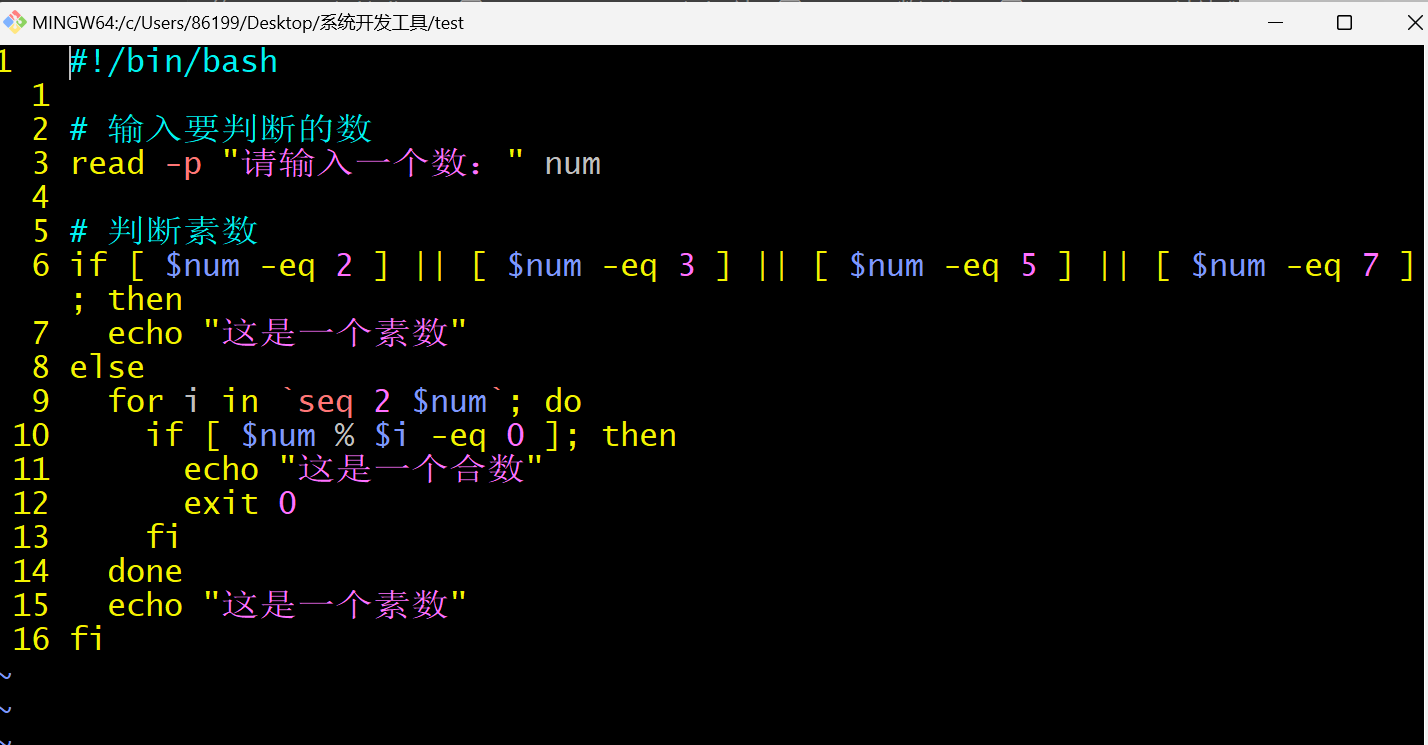
\includegraphics[width=1\textwidth]{shell.png}
    \caption{判断是否为素数}
\end{figure}



\subsection{\color{red}文本编辑工具Vim}
\subsubsection{\color{green}编辑模式}
\begin{itemize}
    \item[-] 正常模式:默认模式,输出esc回到正常模式,移动光标
    \item[-] 插入模式:在正常模式下输入i,进入插入模式,在插入模式下可输入文本
    \item[-] 替换模式:在正常模式下输入R,进入替换模式,替换文本
    \item[-] 可视化模式:在正常模式下输入v,进入可视化模式,可选中文本
    \item[-] 命令模式:在正常模式下输入:,进入命令模式,可执行命令
\end{itemize}
\subsubsection{\color{green}基础命令}
\begin{itemize}
    \item 保存文件: w 
    \item 退出:q
    \item 移动光标:h,j,k,l代表左,上,下,右
    \item 删除: x
    \item 追加文本: a,会同时进入插入模式 
    \item 撤销命令: u;取消撤销: U
    \item 粘贴命令:p
    \item 查找配对的括号:\%
    \item 执行外部命令:!
    \item 在下方插入新行:o;在上方插入新行:O

\end{itemize}
\subsubsection{\color{green}操作符}
\begin{itemize}
    \item d 删除
    \item y 复制
    \item r 替换
    \item / 查找
\end{itemize}
\subsubsection{\color{green}数量符}
    \begin{itemize}
        \item w 从当前光标到下一个单词起始
        \item \$ 从当前光标到行末
        \item 0 从当前光标到行首
        \item e 从当前光标到单词末尾
        \item 数字可以与数量符组
    \end{itemize}
利用vim进行批量操作

\begin{figure}[h]
    \centering
    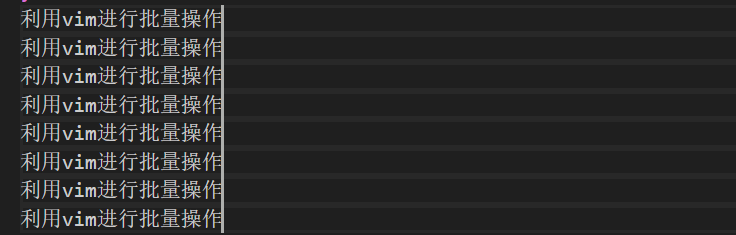
\includegraphics[width=1\textwidth]{vim.png}
    \caption{vim进行批量操作}
    
\end{figure}
\subsection{\color{red}数据整理}
\subsubsection{\color{green}sed流编辑工具}
\begin{itemize}
    \item 命令
        \begin{itemize}
            \item insert 插入
            \item append 追加
            \item delete 删除 
            \item copy 复制
            \item substitute替换
            \item print 打印
        \end{itemize}
    \item 操作
        \begin{itemize}
            \item -e 表达
            \item -i 直接作用文件,生成备份
            \item -n 忽略缓冲区
            \item -f 读取多个文件
        \end{itemize}
\end{itemize}
\begin{figure}[h]
    \centering
    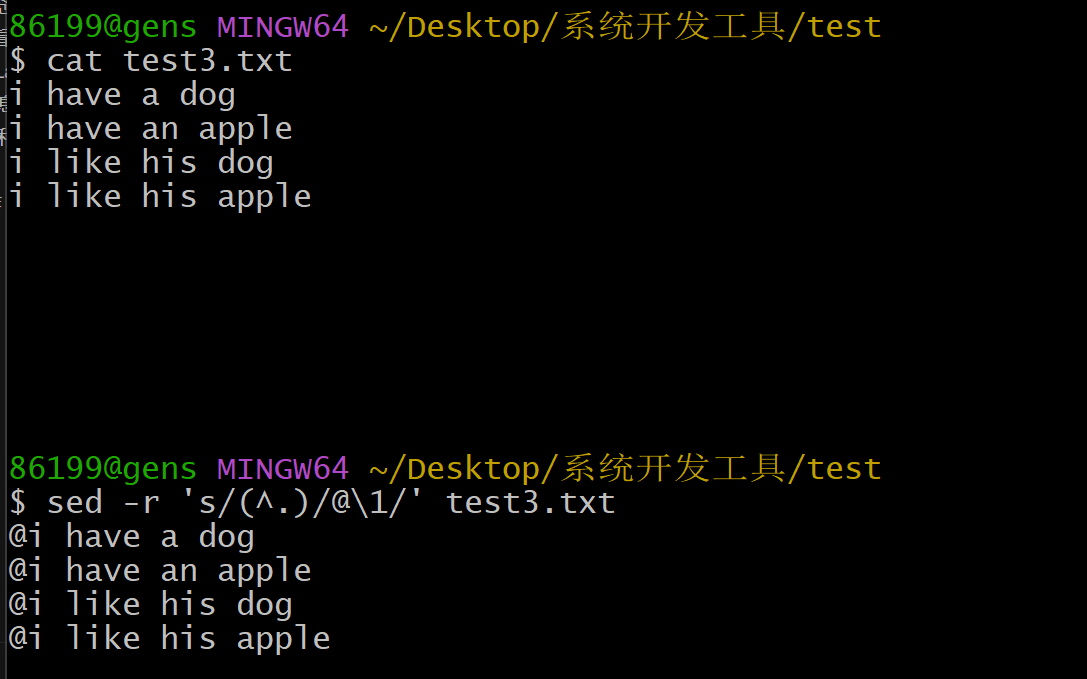
\includegraphics[width=0.8\textwidth]{sed.png}
    \caption{sed和正则替换文件内容}
\end{figure}
\subsubsection{\color{green}正则表达式}
\begin{itemize}
    \item 限定符
        \begin{itemize}
                \item ? 前面的字符出现0此或1次
                \item * 前面的字符出现0次或多次
                \item + 前面的字符出现1次或多次
                \item {num} 前面的字符出现num次,也可以是范围
        \end{itemize}

    % \item 逻辑符
    %     \begin{itemize}
    %         \item \text{langle}  \rangle 分隔
    %         \item \| 或
    %     \end{itemize}
    \item 定位符
        \begin{itemize}
            \item . 代表任何一个字符
            \item ? 可取消贪婪
            \item \$ 只匹配行尾
            % \item \^ 只会匹配行首
        \end{itemize}
    \item 元字符
        \begin{itemize}
            \item \textbackslash{}d 数字字符\\ \textbackslash{}D 非数字字符 
            \item \textbackslash{}w 单词字符(英文、数字、下划线)\\ \textbackslash{}非数字字符
            \item \textbackslash{}s 空白符\\ \textbackslash{} S 非空白符
        \end{itemize}
\end{itemize}

\begin{figure}[h]
    \centering
    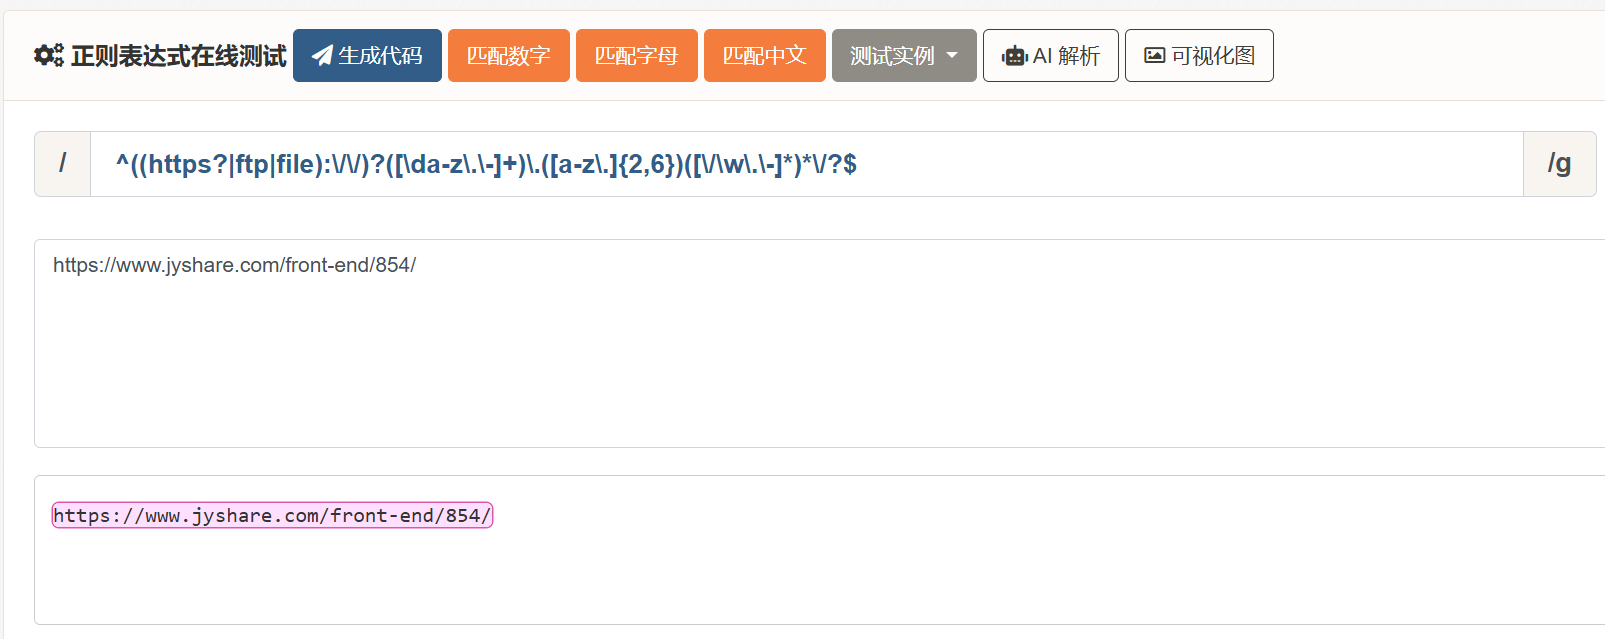
\includegraphics[width=0.8\textwidth]{RegEx.png}
    \caption{匹配网址}

    
\end{figure}
\section{\underline{\color{blue}实验心得}}
通过本次实验,我学会了用shell命令行进行文件操作,学习了脚本编写的基本语法\\
我了解了新的文本编辑工具vim,并将其配置到了我的vscode中,开始订制了自己的vimrc设置文件\\
我认识了流编辑工具sed,学习了正则表达式的基本语法,并学会了用正则表达式进行匹配搜索和替换



% \newpage

% \begin{thebibliography}{99}
%     \bibitem{label1}Anita,ekjfisfjs
%     \bibitem{label2}Bieat,sfsdfwegbraref
% \end{thebibliography}
\end{document}
